\documentclass{article}

\usepackage{iclr2027_conference}
\usepackage[T1]{fontenc}
\usepackage{times}
\usepackage{graphicx}
\usepackage{booktabs}
\usepackage{amsmath}
\usepackage{url}

\renewcommand{\topfraction}{0.95}
\renewcommand{\bottomfraction}{0.9}
\renewcommand{\textfraction}{0.05}
\renewcommand{\floatpagefraction}{0.8}

\graphicspath{{../figures/}{../figures/appendix/}}

\title{Do AI Weather Models Lose Skill in the Tails?\\
A Station-Based Comparison of Global and Regional Systems}

\author{Anonymous Authors}

% Keep \iclrfinalcopy disabled for double-blind review.

\begin{document}
\maketitle

\begin{abstract}
AI weather models are often reported to underpredict extremes, but most
evidence comes from deterministic global systems verified against reanalysis.
We compare eleven learned and numerical alternatives to ECMWF IFS over ten
months. Wind and temperature use 667 European stations at 6--48\,h leads;
solar radiation uses a separate European station panel and hourly leads. Regimes
are fixed by an ERA5 1991--2020 climatology. After a
rolling domain-mean bias correction applied identically to every system, all
five global learned systems lose 2.7--6.8 points of relative MAE skill from all
conditions to the $>$P95 regime in both variables, as does the ECMWF ENS
mean. Under these fixed climatological regimes, two regional generative
systems and the deterministic global numerical models do not. Without
correction, both regional systems still gain and four of five global learned
systems still lose temperature tail skill, but several wind rankings change.
Bias conditioned on the observation points toward the centre
for every system, as expected for imperfect forecasts. When conditioning on
the forecast instead, high-tail temperature bias is within
$0.3\,^{\circ}$C of zero for every system, while wind reveals larger
model-specific differences. The station-verified tail deficit is therefore
reproduced for the tested global learned cohort under fixed climatological
regimes, weakens under in-window percentiles, and is not uniform across
learned forecasting systems. The solar-specific Helios model is strongest in
both irradiance tails but loses skill in the centre of the distribution,
showing that specialization redistributes rather than uniformly improves
skill.
\end{abstract}

\section{Introduction}

Data-driven weather models now match or outperform operational numerical
systems on standard forecast scores
\citep{bi2023pangu,lam2023graphcast,bouallegue2024rise}. Their behaviour in
the tails remains contested. Models trained with mean squared error are
expected to regress toward the conditional mean and smooth sharp gradients
\citep{olivetti2024,bonavita2024limitations}. Storm Ciar\'an forecasts
underestimated peak winds \citep{charltonperez2024}, and errors for
record-breaking heat, cold, and wind are systematically larger than IFS HRES
\citep{zhang2026records}. Other events and regions show
learned systems matching or exceeding numerical forecasts
\citep{olivetti2024extremes,pasche2025validating}.

Three design choices limit what can be inferred from this literature. First,
many studies verify ERA5-trained models against ERA5, whereas station
observations expose local variability absent from a gridded target
\citep{jin2024weatherreal,gupta2025mausam}. Second, most comparisons concern
global deterministic regression systems. Regional learned models and
proper-score-trained ensembles have been studied individually
\citep{nipen2026bris,lang2026aifscrps}, but rarely under the same
station-based protocol. Third, evaluation only on cases where the observation
is extreme creates the forecaster's dilemma: it rewards high-amplitude
forecasts and induces apparent regression toward the centre for any imperfect
forecast \citep{murphy1987framework,lerch2017forecasters}.

We therefore ask a bounded question: \emph{after the same rolling mean-bias
correction is applied to every forecast, do learned systems lose relative MAE
skill from all conditions to the tails, and does that loss separate learned
from numerical forecasting?} We compare global and regional systems over
Europe for 10\,m wind and 2\,m temperature. Observed-value regimes use fixed
ERA5 1991--2020 thresholds at each station, day of year, and hour. We report
absolute skill relative to IFS, the change from all-condition to tail skill,
raw-versus-corrected sensitivity, and both observation- and
forecast-conditioned bias.

The answer is structured rather than uniform. Under fixed climatological
regimes and after correction, every tested global learned system loses
relative skill from all conditions to the upper tail in both variables. The
ECMWF ENS mean behaves similarly. The two
regional generative systems and deterministic global numerical models do not,
although the regional wind result is sensitive to bias correction and regime
definition. This
pattern does not isolate a cause: domain, resolution, training data, ensemble
averaging, and model provenance are confounded. It does identify which
systems reproduce the reported tail deficit and which provide
counterexamples.

\section{Related work}

\paragraph{Evidence at extremes.}
Storm Ciar\'an evaluations found that FourCastNet, Pangu-Weather, and
GraphCast reproduced the synoptic structure but underestimated peak winds
\citep{charltonperez2024}. Record-breaking heat, cold, and wind were also
forecast less accurately by GraphCast, Pangu-Weather, and FuXi than by IFS
HRES \citep{zhang2026records}. Systematic results are more mixed. Against
ERA5, GraphCast and Pangu-Weather compete with HRES in many regions but lose
for warm extremes over Europe \citep{olivetti2024extremes}. At European
SYNOP stations, Pangu-Weather discriminates summer warm events well, while
still missing some intensity extremes \citep{bouallegue2024rise}. Impact
case studies likewise find learned forecasts competitive locally on one
heatwave and superior on a compound winter storm, but weaker under other
aggregations \citep{pasche2025validating}.

\paragraph{Objectives and regional systems.}
Grid-point regression incurs a double penalty when a displaced feature is
penalized both where it is missing and where it appears. This can reduce the
effective resolution of learned forecasts
\citep{subich2025doublepenalty}. Generative models instead learn a
distribution of plausible states \citep{price2024gencast,pathak2026stormcast}.
AIFS ENS optimizes an objective based on a proper score
\citep{lang2026aifscrps}, while regional systems increase spatial resolution
over a limited domain \citep{nipen2026bris,molinaro2026downscaling}. In this
study every ensemble is evaluated through its mean. The comparison therefore
tests the tail error of a point summary, not whether a probabilistic
objective recovers the distribution of extremes.

\paragraph{Station verification.}
WeatherReal \citep{jin2024weatherreal} and MAUSAM
\citep{gupta2025mausam} show that near-surface errors against observations
can substantially exceed errors against reanalysis. We use the StationBench
stack \citep{wagner2025stationbench}, but define regimes from an external
climatology rather than from the scored period.

\paragraph{Conditional verification.}
Forecast verification admits two complementary factorizations: observations
conditioned on forecasts diagnose reliability, while forecasts conditioned
on observations describe discrimination \citep{murphy1987framework}.
Restricting a conventional score to extreme observations is not a proper
forecast comparison and can favour exaggerated amplitude
\citep{lerch2017forecasters}. We retain observed regimes because they directly
measure error on the realized tail, but interpret them comparatively and add
forecast-conditioned bias as a reliability diagnostic.

\section{Methods}\label{sec:methods}

\subsection{Forecast systems and observations}

Track A compares ten wind and temperature alternatives with ECMWF IFS: ECMWF ENS, NOAA GFS, DWD
ICON Global, ECMWF AIFS \citep{lang2024aifs}, ECMWF AIFS ENS
\citep{lang2026aifscrps}, Microsoft Aurora \citep{bodnar2025aurora}, and Jua
EPT-2 Reasoning, EPT-2e, EPT-2 HRRR, and EPT-2.1 Europa
\citep{molinaro2025ept2,jua2025hrrr,jua2026europadocs}. AIFS ENS is scored
as a 51-member mean; EPT-2 HRRR and EPT-2.1 Europa are diffusion-based
ensembles. The solar comparison additionally includes the solar-specific
EPT-2.1 Helios \citep{jua2026helios}. Track B adds the regional numerical ICON-EU on the
March--June 2026 window. Appendix~\ref{app:details} lists model class, output,
domain, and archive provenance.

Forecasts are verified at 667 stations with complete climatological
thresholds across thirteen European countries. The scored panel contains 227
stations in France and 8--81 in each other country
(Table~\ref{tab:stationcounts}). Gridded forecasts are bilinearly interpolated
to station locations. The EPT-2 family was pretrained partly on SYNOP and
METAR networks \citep{jua2026benchmarks}, so station-network independence is not claimed; the
forecast-valid period follows the published pretraining period. Model
results are out of sample with respect to model development, but station
overlap remains a limitation.

Track A covers 1 September 2025--30 June 2026. Wind and temperature use all
00, 06, 12, and 18 UTC initializations and the common 6, 12, \ldots, 48\,h
lead grid. A model and IFS are pooled on their common country, regime, lead,
and initialization-time cells, using the same station--initialization--lead
pairs within each cell. Results are sample-weighted across countries, so
France contributes 39\% of upper-wind-tail and 48\% of
upper-temperature-tail samples.

Solar radiation is evaluated on a separate quality-controlled panel over the
same period and on hourly leads from 1 to 48\,h. Regime-stratified results use
543 stations with fixed thresholds across nine countries. The model
set contains Helios, Europa, HRRR, EPT-2e, EPT-2 Reasoning, ICON Global, GFS,
and IFS. All reported solar results are likewise out of sample.

\subsection{Climatological regimes}

For each station, calendar day, and UTC hour, we estimate ERA5 P5, P25, P75,
and P95 over 1991--2020 using a cyclic $\pm15$-day window. Each threshold is
estimated from 930 values. Forecast--observation pairs are assigned to a
regime using the observation. The bands are $<$P5, P5--P25, P25--P75,
P75--P95, and $>$P95, together with all conditions.

These are anomaly regimes, not impact thresholds. Across station--time cells,
the median wind P95 is 6.6\,m\,s$^{-1}$; median temperature P95 and P5 are
$16.0\,^{\circ}$C and $5.6\,^{\circ}$C. Wind tails are approximately
symmetric (10.2\% above P95 and 9.2\% below P5), consistent with greater
point-observation variance. Temperature is asymmetric (13.5\% above P95 and
3.2\% below P5), reflecting a warm evaluation period relative to 1991--2020.
We therefore use percentile notation rather than physical labels.

\subsection{Skill, debiasing, and uncertainty}

For model $m$ in evaluation cell $c$, MAE skill relative to IFS is
\begin{equation}
S_{m,c}=100\left(1-\frac{\operatorname{MAE}_{m,c}}
{\operatorname{MAE}_{\mathrm{IFS},c}}\right).
\end{equation}
Positive values indicate lower MAE than IFS. Ensemble systems are reduced to
their means; MAE of the mean does not assess ensemble spread or calibration.

The primary comparison removes a rolling domain-mean offset. For each model,
week, initialization hour, and lead, we average errors over all European
stations during the preceding four valid weeks and subtract that scalar from
the next week's forecasts. The correction does not use the observed regime,
but a uniform shift can have a large regime-dependent effect. Raw and
corrected results are therefore reported together. The correction is causal
with respect to valid time; up to one forecast lead of its training window can
postdate forecast issuance.

We pool MAE linearly by sample count and discard country--lead cells with
fewer than 100 pairs. Uncertainty is one leave-one-month-out jackknife
standard error, computed with the same linear pooling as the point estimate.
Track A has ten monthly blocks and Track B four. These errors describe
month-to-month sensitivity of the pooled estimate, not country-level
dispersion or a multiple-testing-adjusted confidence interval.

\subsection{Robustness and conditional diagnostics}

Our direct test of tail degradation is
$\Delta S=S_{>P95}-S_{\mathrm{all}}$. Negative values mean that a system loses
skill relative to IFS when moving from all conditions to the observed upper
tail. We report $\Delta S$ for raw and corrected forecasts. Appendix
\ref{app:robustness} additionally replaces the station--day--hour
climatological regimes with one country-level percentile distribution over
the evaluation window. This selects absolute rather than local-anomaly tails.

Observation-conditioned bias,
$E[F-Y\mid Y\in\mathcal{R}]$, is expected to point toward the centre for an
imperfect forecast. We therefore also report forecast-conditioned bias,
$E[F-Y\mid F\in\mathcal{R}]$, using the same fixed thresholds. The latter is
zero for a conditionally unbiased point forecast and provides the reliability
view missing from an observed-tail score.

\section{Results}\label{sec:results}

\subsection{A structured tail penalty}

Figure~\ref{fig:tailpenalty} reports the change from all-condition to upper-tail
skill. After correction, every global learned system loses 2.7--6.8 points in
both variables. The ECMWF ENS mean loses 2.5 points in wind and 4.4 in
temperature. HRRR gains $1.8\pm0.7$ points in wind and $7.5\pm2.1$ in
temperature; Europa's changes are $+0.5\pm0.8$ and $+3.6\pm1.2$.
Deterministic ICON Global and GFS gain 0.9--11.8 points. Learned versus
numerical forecasting does not separate the outcomes, but global learned
systems and ensemble means form a consistent negative group.

The correction matters. On raw wind forecasts, Europa loses 6.2 points from
all conditions to $>$P95, HRRR is approximately unchanged, and GFS gains 22
points. For temperature, both regional learned systems retain positive tail
changes before and after correction, while raw AIFS gains 0.9 points in the
upper tail. The regional exception is therefore more robust to correction in
temperature than wind, whereas the global learned penalty is more robust in
wind. No tail ranking is reported independently of the correction.

\begin{figure}[t]
\centering
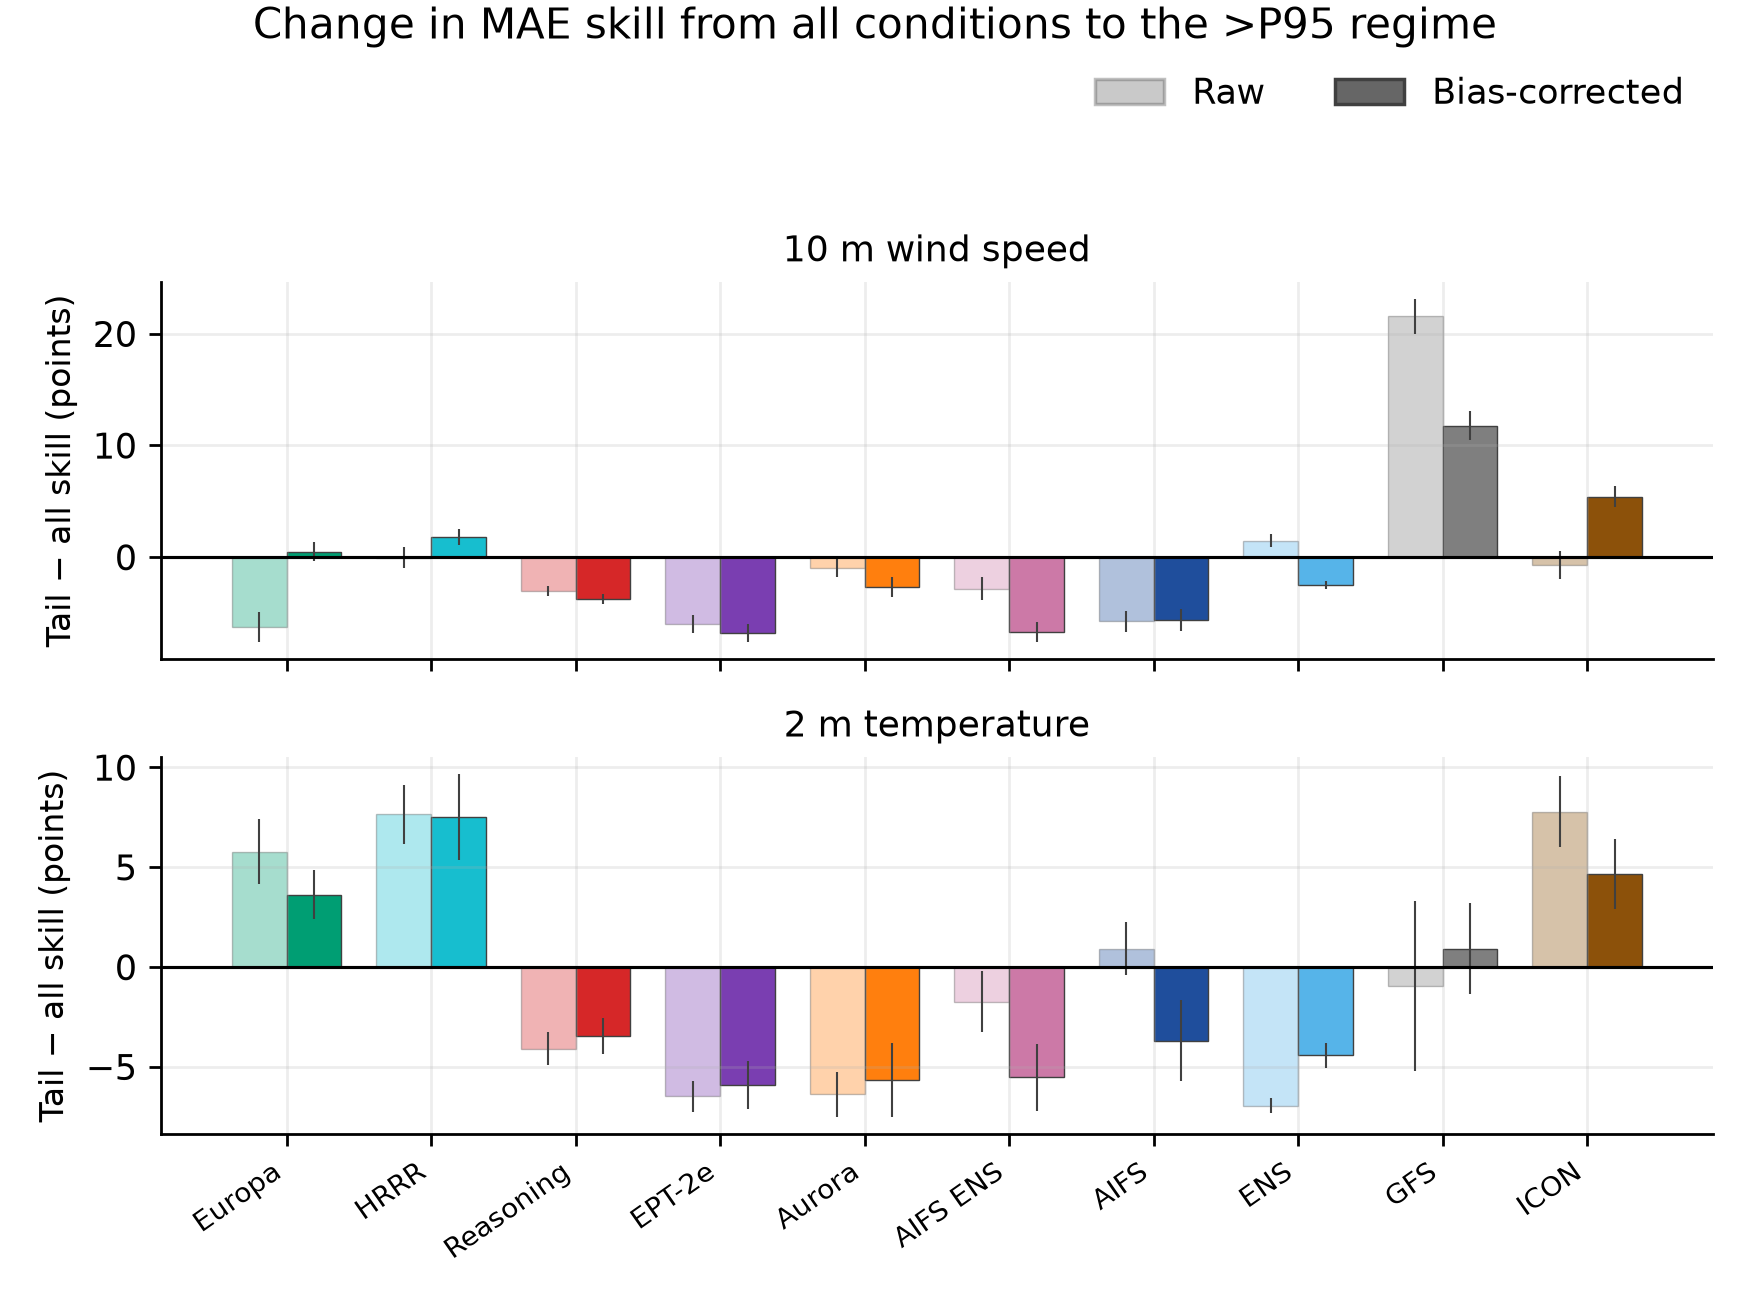
\includegraphics[width=.96\textwidth]{fig_tail_penalty.png}
\caption{Change in MAE skill from all conditions to the observed $>$P95
regime, 6--48\,h. Negative values indicate relative degradation in the tail.
Light bars are raw forecasts; dark bars apply the common rolling domain-mean
bias correction. Error bars give one leave-one-month-out jackknife standard
error for the tail-minus-all difference.}
\label{fig:tailpenalty}
\end{figure}

\subsection{Absolute skill and AIFS ENS}

Absolute corrected skill remains heterogeneous
(Figure~\ref{fig:skillbars}). Europa and HRRR are ahead of IFS in the upper
wind and temperature tails; ICON Global is also ahead. All global learned
systems are behind IFS in upper-tail wind. In temperature, EPT-2 Reasoning
remains slightly positive while AIFS, AIFS ENS, Aurora, and EPT-2e are
negative. Below temperature P5, those four systems lose 20--24\% under the
climatological definition, although this magnitude is not robust to the
threshold definition.

\begin{figure}[t]
\centering
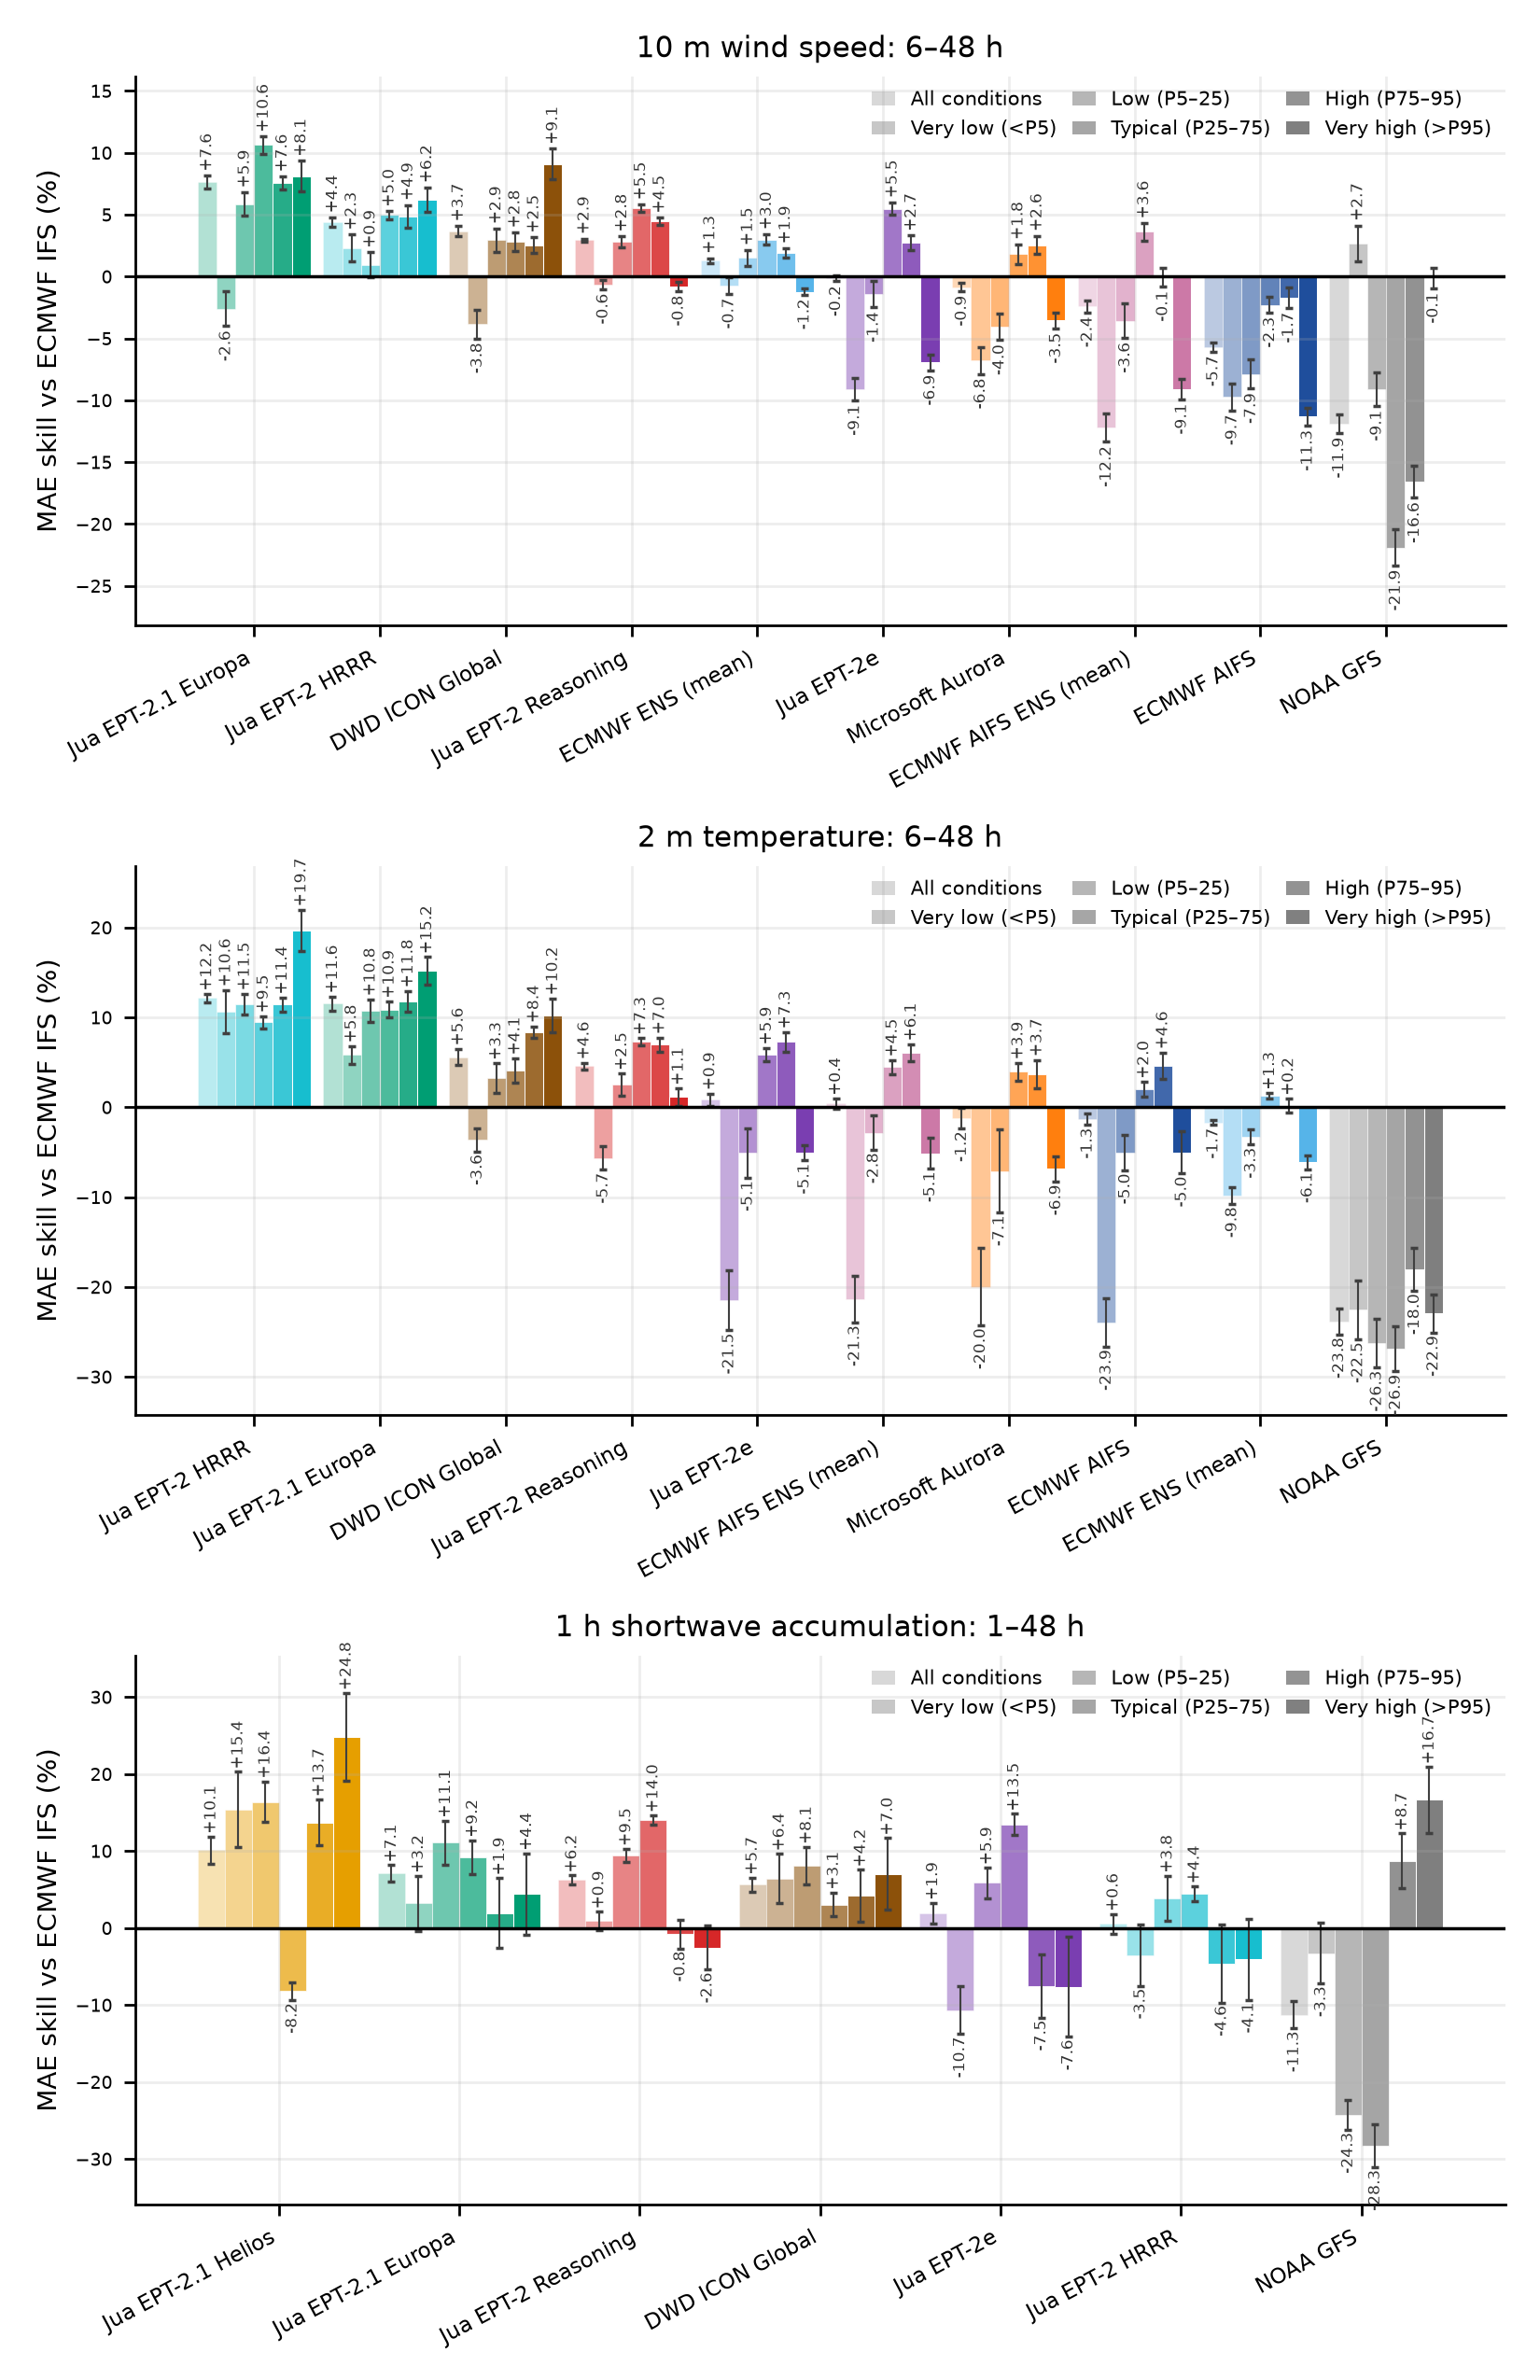
\includegraphics[width=.94\textwidth]{fig3_headline_bars.png}
\caption{Bias-corrected Track A MAE skill against ECMWF IFS by
observation-conditioned climatological regime. Wind and temperature pool
6--48\,h; solar pools 1--48\,h. Error bars give one leave-one-month-out
jackknife standard error.}
\label{fig:skillbars}
\end{figure}

AIFS ENS narrows the all-condition wind deficit of deterministic AIFS
($-2.4\%$ versus $-5.7\%$) but remains behind IFS above the wind P95
($-9.1\%$). Against the like-for-like ECMWF ENS mean, it is 7.9 points worse
in that regime. For temperature, AIFS ENS and the ECMWF ENS mean have similar
upper-tail skill ($-5.1\%$ and $-6.1\%$). This result constrains the
ensemble mean only: it does not test whether proper-score training improves
tail probabilities.

\subsection{Solar specialization}

Solar results reinforce the need to compare regimes rather than one mean
score. Helios leads all conditions ($+10.1\pm1.7\%$), P5--P25 irradiance
($+16.4\pm2.7\%$), and the $>$P95 regime ($+24.8\pm5.7\%$), but loses
$8.2\pm1.2\%$ in the central P25--P75 band. EPT-2 Reasoning instead leads
that central band at $+14.0\pm0.6\%$. GFS shows the same redistribution in
more extreme form: $+16.7\%$ above P95 and $-28.3\%$ in the centre.
Observation-conditioned tail skill therefore reflects amplitude as well as
accuracy, consistent with the forecaster's dilemma.

\subsection{Sensitivity to thresholds and horizon}

Changing from fixed climatological thresholds to in-window percentiles
reduces several large tail magnitudes. In particular, AIFS ENS skill below
temperature P5 changes from $-21.3\%$ to $-0.3\%$, while its upper-tail
wind and temperature results remain negative. The regional systems remain
positive in both upper tails, but EPT-2 Reasoning becomes positive under the
in-window definition. Under that definition, the wind penalties of AIFS and
Aurora shrink to within one standard error of zero ($-0.3$ and $-0.2$
points), the temperature changes of Aurora and EPT-2 Reasoning turn positive,
and the regional wind gain reverses to $-2$ to $-3$ points. The uniform sign
is a property of the fixed
climatological regimes. The claim is therefore about a structured tendency,
not an invariant ordering for every definition
(Table~\ref{tab:thresholdsensitivity}).

\subsection{What conditional bias shows}

The left column of Figure~\ref{fig:conditional} reproduces the displacement
expected when conditioning an imperfect forecast on the observation. Every
system overpredicts low observations and underpredicts high observations.
The common sign is not evidence that models themselves shrink extremes.

\begin{figure}[t]
\centering
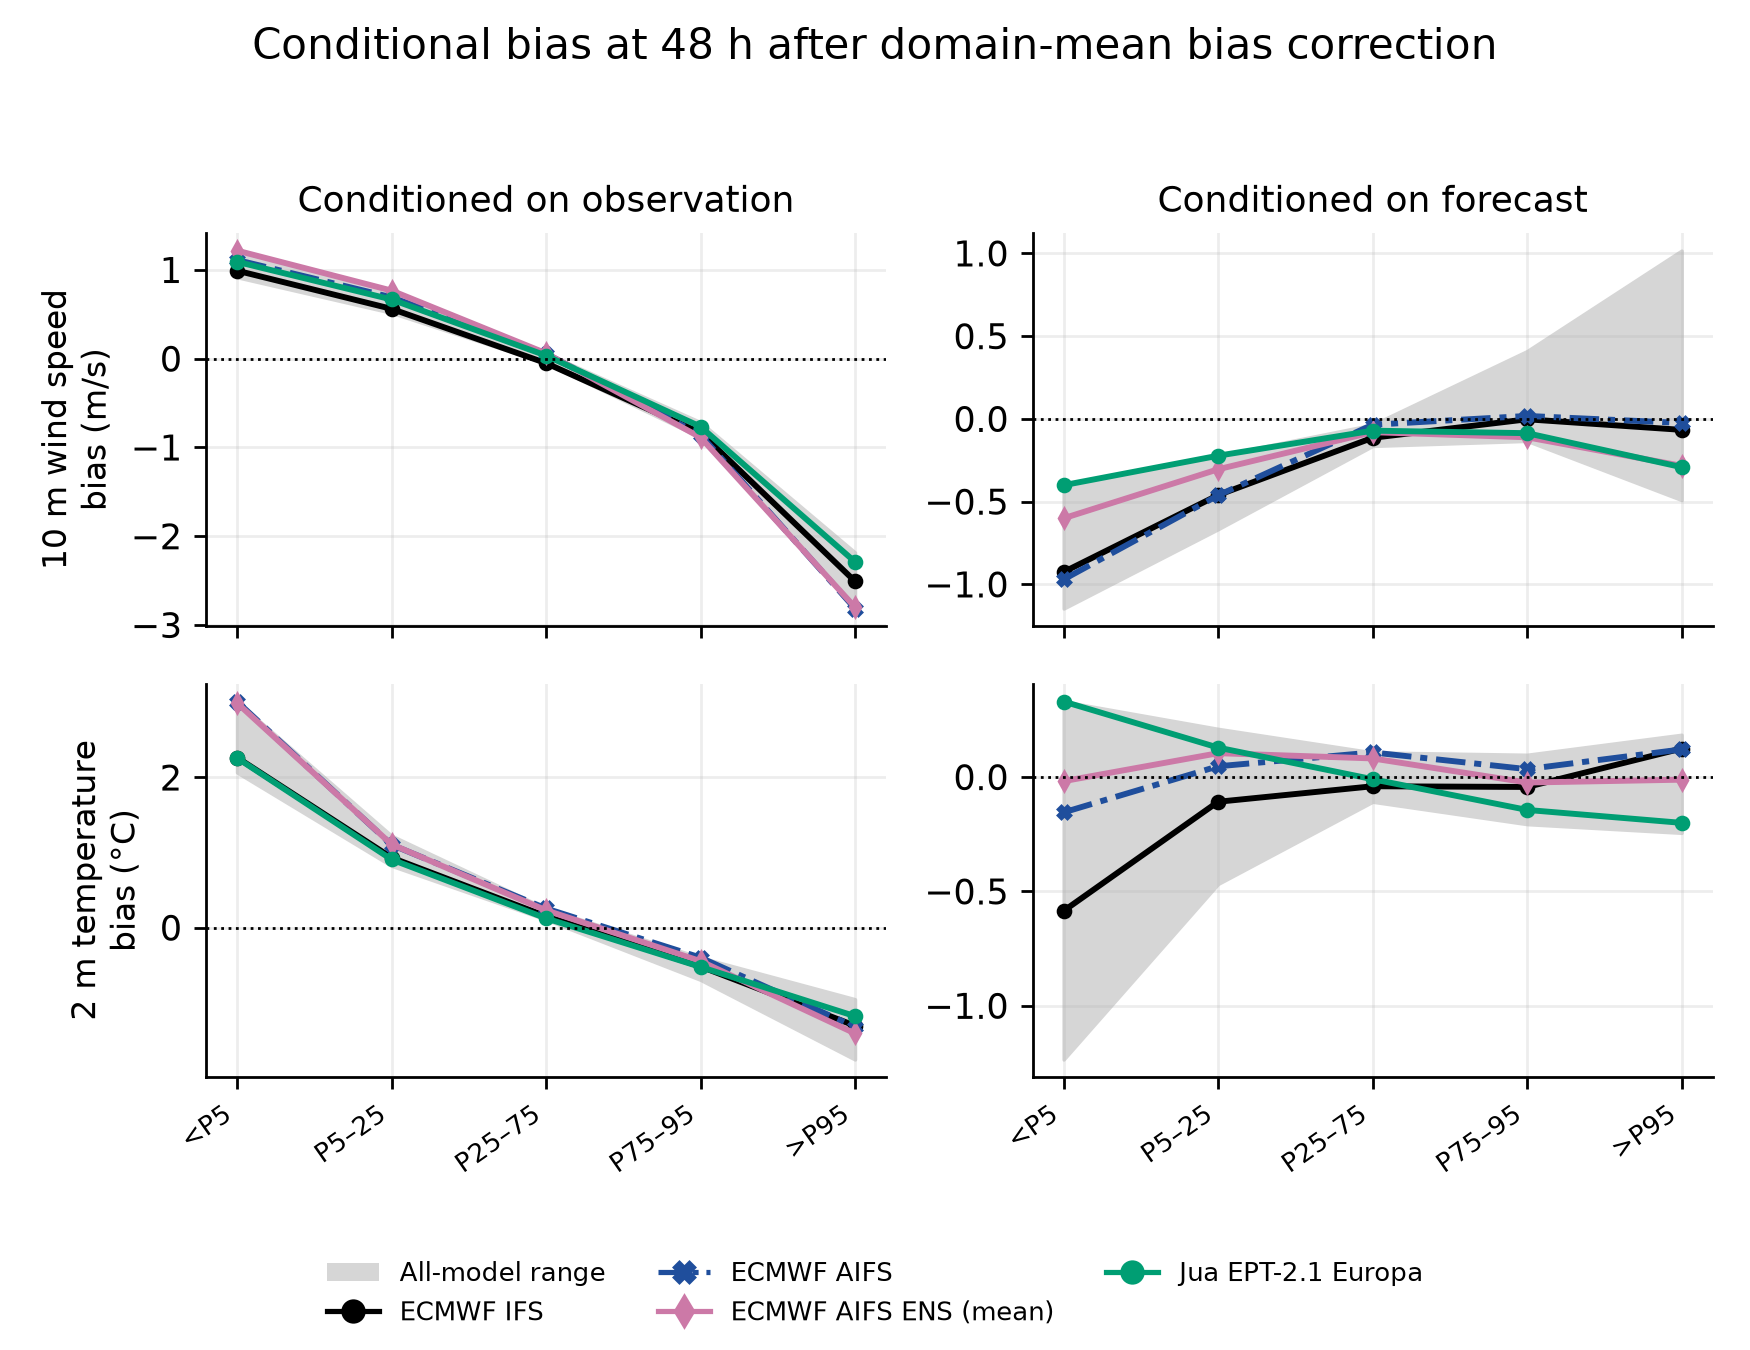
\includegraphics[width=.96\textwidth]{fig_conditional_bias_comparison.png}
\caption{Forecast-minus-observation bias at 48\,h after domain-mean bias
correction. Left: regimes defined by the observation. Right: regimes defined
by the forecast. Grey bands span all models; lines highlight IFS, deterministic
AIFS, AIFS ENS, and Europa. The columns use different vertical scales.}
\label{fig:conditional}
\end{figure}

The forecast-conditioned view is different. Above the temperature P95, every
system lies within $0.3\,^{\circ}$C of zero bias. Above the wind P95, most
systems lie within 0.5\,m\,s$^{-1}$, while GFS overpredicts by
1.0\,m\,s$^{-1}$. Forecasts in the lowest wind regime are too low by
0.4--1.1\,m\,s$^{-1}$. Thus the observation-conditioned fingerprint mainly
reflects the verification factorization. Forecast-conditioned errors are
smaller; some are shared, such as underprediction in the lowest wind regime,
while upper-tail wind errors differ by model.

\subsection{Regional corroboration}

On Track B, EPT-2.1 Europa has $+6.5\pm0.3\%$ all-condition wind skill,
compared with $+4.6\pm0.4\%$ for ICON-EU. Their upper-wind-tail estimates,
$+9.3\pm1.5\%$ and $+10.4\pm1.8\%$, are close relative to a four-month
jackknife. The learned and numerical regional systems are also positive in
the upper temperature tail. This comparison supports a regional exception
but does not isolate resolution, model design, or provenance.

\section{Discussion}

The evidence supports a narrower conclusion than a binary claim about AI
weather models. After domain-mean bias removal, every tested global learned
system loses relative MAE skill from all conditions to the upper wind and
temperature tails under the fixed climatological regimes. Two regional learned systems do not, and regional
ICON-EU behaves similarly. Neither domain nor model class alone separates the
outcomes: the negative group consists of global learned systems and ensemble
means, and the positive group of regional learned systems and deterministic
global numerical models. The experiment cannot separate resolution and
domain from training objective, ensemble averaging, model family, or vendor.

Bias correction is part of this conclusion, not a technical footnote. It
removes an offset that operational users can estimate from prior valid times,
but it also
changes several upper-wind-tail rankings and reverses the sign of the AIFS
and AIFS ENS temperature comparisons. Reporting raw and corrected values
bounds the claim: the global learned penalty appears in nine of ten raw
model--variable cells, whereas the regional wind exception is not visible
without correction.

The conditional analysis resolves a second ambiguity. Conditioning on the
realized observation necessarily creates apparent movement toward the centre,
so its sign should not be interpreted as a model defect. The useful
information is the cross-model magnitude and the forecast-conditioned
reliability view. For upper-tail temperature, the latter is near zero across
systems even when observation-conditioned MAE differs substantially.

Finally, ensemble means are point summaries. The similar upper-temperature
tail losses of AIFS ENS and ECMWF ENS are consistent with ensemble averaging,
not evidence against proper-score training. Probabilistic scores are required
to evaluate the objective for which these systems were trained.

\section{Limitations}

Some authors have a potential conflict of interest with a subset of the
evaluated systems; details are withheld for double-blind review and will be
disclosed in the camera-ready. Public
documentation states that the EPT-2 family was
pretrained partly on SYNOP and METAR networks \citep{jua2026benchmarks}, so station identity may overlap
training even though the scored forecast period is later. All reported
results are out of sample with respect to model development. Potential vendor
effects remain, and no causal attribution is made from the regional
counterexamples.

The scored network is geographically uneven: France contributes 39--48\% of
upper-tail pairs, while several countries have fewer than twenty stations.
Monthly jackknife errors do not capture this spatial heterogeneity. IFS,
AIFS, and AIFS ENS changed operational versions on 12 May 2026
\citep{ecmwf2026cycle50r1}. The analysis treats
each named product as one forecast system and does not isolate version
effects.

Results are limited to Europe, ten months, and primarily 6--48\,h. The
climatological upper-temperature regime contains 13.5\% of evaluation hours
and is not an impact-defined extreme. Threshold-definition sensitivity is
reported because it materially changes magnitudes.

All ensembles are evaluated through their means. The study does not assess
calibration, spread, spatial coherence, or event probabilities. The
observed-tail MAE comparison is also subject to the forecaster's dilemma and
should not be read as a proper probabilistic evaluation.

\section{Conclusion}

At European stations, 6--48\,h leads, and fixed climatological regimes, the
tested global learned systems all lose relative MAE skill from all conditions
to the upper wind and temperature tails after common domain-mean bias removal.
Regional learned and numerical systems provide counterexamples, although the
regional wind result depends on the correction and regime definition. The
evidence therefore supports a structured contrast
in which global learned systems and ensemble means lose tail skill while
regional learned and deterministic global numerical systems do not, rather
than a uniform learned-versus-numerical divide. Observation-conditioned
displacement toward the centre is expected
for any imperfect forecast; forecast-conditioned bias shows much smaller
model-specific reliability errors. These conclusions concern point summaries
and do not extend to probabilistic calibration.

\clearpage
\subsubsection*{Reproducibility statement}
The anonymous package reproduces score-based tables and figures from compact
aggregate data and includes the extraction and aggregation code. Rebuilding synoptic
aggregates from station-level errors requires access to the read-only
verification warehouse and is not available to third parties. The package
does not release station identities or per-station series. Every preserved
compact input is integrity-checked and recorded in the aggregate status file.

\subsection*{AI use statement}
Generative AI tools were used to review experimental methodology, challenge
claims, assist with software changes, inspect generated results, search
literature, suggest paper structure, and draft and edit manuscript text. They
were not used to generate synthetic observations, formulate or prove
mathematical claims, or replace the authors' quantitative analysis. The
authors checked AI-assisted code through executable tests and regenerated
artifacts, checked numerical claims against aggregate data, reviewed the
cited literature and all manuscript text, and take responsibility for the
final content.

\bibliography{references}
\bibliographystyle{iclr2027_conference}

\appendix
\section{Model and data details}\label{app:details}

\subsection{Forecast systems}
Table~\ref{tab:models} lists the systems. All reported results are out of
sample with respect to model development. IFS, AIFS, and AIFS ENS changed
operational versions on 12 May 2026 \citep{ecmwf2026cycle50r1}; the analysis
treats each named product as one system and does not isolate version effects.

\begin{table}[h]
\caption{Forecast systems. Ensemble systems are evaluated through their
means. ICON-EU appears only in Track B; Helios only in the solar comparison.}
\label{tab:models}
\centering\small
\resizebox{\textwidth}{!}{%
\begin{tabular}{llll}
\toprule
Model & Class & Output & Domain \\
\midrule
ECMWF IFS (reference) & physical & deterministic & global \\
ECMWF ENS & physical & ensemble & global \\
NOAA GFS & physical & deterministic & global \\
DWD ICON Global & physical & deterministic & global \\
DWD ICON-EU & physical & deterministic & regional \\
ECMWF AIFS & regression AI & deterministic & global \\
ECMWF AIFS ENS & proper-score AI & 51-member ensemble & global \\
Microsoft Aurora & regression AI & deterministic & global \\
Jua EPT-2 Reasoning & regression AI & deterministic & global \\
Jua EPT-2e & regression AI & ensemble & global \\
Jua EPT-2 HRRR & generative AI & ensemble & regional \\
Jua EPT-2.1 Europa & generative AI & ensemble & regional \\
Jua EPT-2.1 Helios & solar AI & deterministic & regional \\
\bottomrule
\end{tabular}}
\end{table}

\subsection{Station panel and tracks}
The scored synoptic panel consists of the 667 stations for which fixed ERA5
thresholds are available. Country counts are in
Table~\ref{tab:stationcounts}; the full station catalogue shown in
Figure~\ref{fig:network} is larger and is not the scored count.

\begin{table}[h]
\caption{Synoptic stations contributing to the fixed-climatology analysis.}
\label{tab:stationcounts}
\centering\small\begin{tabular}{@{}lr@{}}
\toprule
Country & Stations with fixed thresholds \\
\midrule
AT & 8 \\
BE & 12 \\
CH & 16 \\
CZ & 11 \\
DE & 67 \\
DK & 12 \\
ES & 40 \\
FR & 227 \\
GB & 74 \\
IT & 81 \\
NL & 13 \\
NO & 31 \\
PL & 75 \\
\midrule
Total & 667 \\
\bottomrule
\end{tabular}

\end{table}

\begin{figure}[h]
\centering
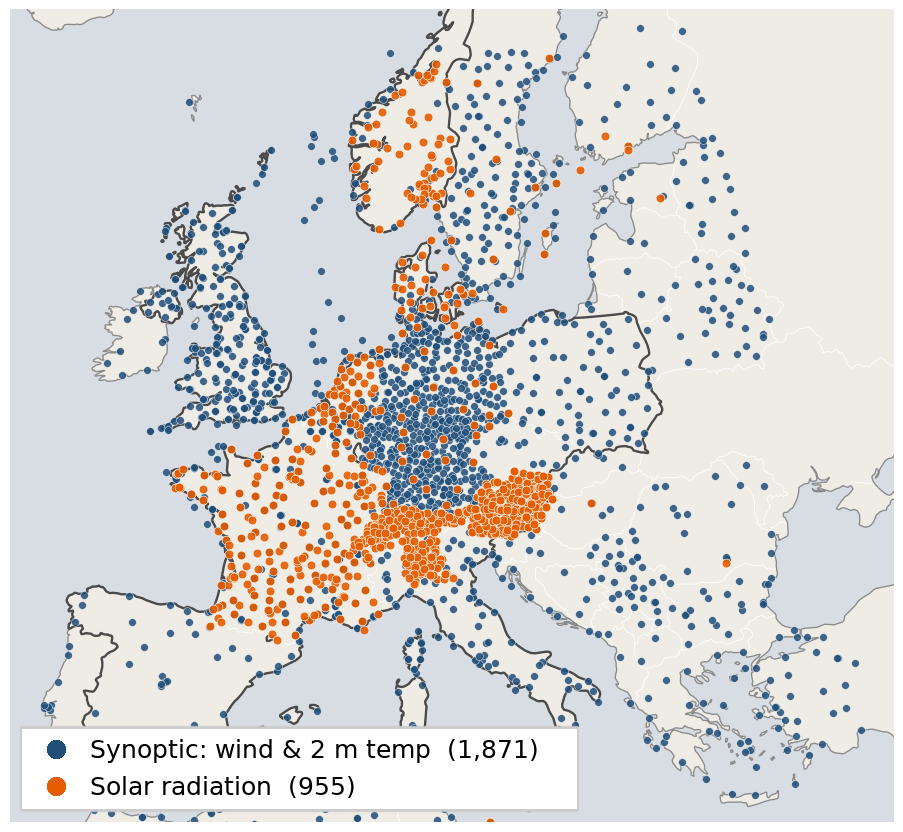
\includegraphics[width=.63\textwidth]{fig1_station_network.png}
\caption{Full station catalogues available to the verification system. Only
stations with fixed climatological thresholds enter the reported wind and
temperature regimes; the solar catalogue is likewise larger than its scored
regime panel.}
\label{fig:network}
\end{figure}

Track A covers 1 September 2025--30 June 2026 over DE, FR, GB, ES, IT, PL,
NL, BE, CH, NO, AT, CZ, and DK. It uses all four daily initialization cycles
and the common six-hourly lead grid from 6 to 48\,h. Track B covers
March--June 2026 and compares the regional systems on their common hourly
lead grid.

Solar radiation uses hourly leads from 1 to 48\,h. Regime-stratified results
use 543 stations with fixed thresholds in BE, CH, DE, DK, ES, FR, IT, NL, and
NO. Austrian catalogue stations were not part of the frozen score extraction;
GB and PL are absent, and CZ lacks fixed solar thresholds. Spain contributes
one station through March 2026, and Italian coverage ends after February.

\subsection{Observed-value regimes}
For each station, calendar day, and UTC hour, ERA5 P5, P25, P75, and P95 are
estimated over 1991--2020 with a cyclic $\pm15$-day window. The five regimes
are assigned from the verifying observation. Because they follow the
day-of-year climatology, they represent local anomalies rather than fixed
physical severity.

\section{Complete Track A results}\label{app:tracka}

\begin{table}[h]
\caption{Bias-corrected Track A MAE skill (\%) against IFS, 6--48\,h, by
wind regime. Parentheses give leave-one-month-out jackknife standard errors.}
\label{tab:skillwind}
\centering\small\resizebox{\textwidth}{!}{\begin{tabular}{@{}lrrrrrr@{}}
\toprule
Model & All & $<$P5 & P5--25 & P25--75 & P75--95 & $>$P95 \\
\midrule
Jua EPT-2.1 Europa & +8.4\,(0.5) & -1.7\,(1.4) & +6.4\,(0.9) & +11.3\,(0.7) & +8.5\,(0.4) & +9.0\,(1.2) \\\addlinespace[0.35em]
Jua EPT-2 HRRR & +4.5\,(0.3) & +2.7\,(1.0) & +1.4\,(0.9) & +5.1\,(0.3) & +4.9\,(1.0) & +6.1\,(0.9) \\\addlinespace[0.35em]
Jua EPT-2 Reasoning & +3.0\,(0.1) & -0.7\,(0.4) & +2.8\,(0.5) & +5.6\,(0.3) & +4.5\,(0.3) & -0.7\,(0.3) \\\addlinespace[0.35em]
Jua EPT-2e & -0.0\,(0.2) & -9.1\,(1.0) & -1.4\,(1.1) & +5.6\,(0.5) & +2.9\,(0.6) & -6.6\,(0.5) \\\addlinespace[0.35em]
Microsoft Aurora & -0.7\,(0.3) & -6.6\,(1.1) & -3.9\,(1.1) & +1.9\,(0.8) & +2.6\,(0.8) & -3.4\,(0.6) \\\addlinespace[0.35em]
ECMWF AIFS & -5.4\,(0.4) & -9.8\,(1.2) & -8.0\,(1.3) & -2.1\,(0.6) & -1.4\,(0.8) & -10.6\,(0.6) \\\addlinespace[0.35em]
ECMWF ENS (mean) & +1.4\,(0.2) & -0.9\,(0.7) & +1.5\,(0.6) & +3.1\,(0.4) & +2.1\,(0.4) & -1.0\,(0.2) \\\addlinespace[0.35em]
NOAA GFS & -11.7\,(0.7) & +1.8\,(1.4) & -9.5\,(1.4) & -21.8\,(1.4) & -16.3\,(1.3) & +0.6\,(0.7) \\\addlinespace[0.35em]
DWD ICON Global & +3.6\,(0.4) & -4.1\,(1.2) & +2.8\,(1.0) & +2.6\,(0.7) & +2.5\,(0.7) & +9.5\,(1.1) \\
\bottomrule
\end{tabular}
}
\end{table}

\begin{table}[h]
\caption{Bias-corrected Track A MAE skill (\%) against IFS, 6--48\,h, by
temperature regime.}
\label{tab:skilltemp}
\centering\small\resizebox{\textwidth}{!}{\begin{tabular}{@{}lrrrrrr@{}}
\toprule
Model & All & $<$P5 & P5--25 & P25--75 & P75--95 & $>$P95 \\
\midrule
Jua EPT-2.1 Europa & +11.6\,(0.8) & +5.8\,(1.0) & +10.8\,(1.2) & +10.9\,(0.9) & +11.8\,(1.2) & +15.2\,(1.5) \\\addlinespace[0.35em]
Jua EPT-2 HRRR & +12.2\,(0.4) & +10.6\,(2.4) & +11.5\,(1.1) & +9.5\,(0.7) & +11.4\,(0.8) & +19.7\,(2.3) \\\addlinespace[0.35em]
Jua EPT-2 Reasoning & +4.6\,(0.4) & -5.7\,(1.3) & +2.5\,(1.2) & +7.3\,(0.4) & +7.0\,(0.8) & +1.1\,(1.0) \\\addlinespace[0.35em]
Jua EPT-2e & +0.9\,(0.7) & -21.5\,(3.3) & -5.1\,(2.8) & +5.9\,(0.7) & +7.3\,(1.1) & -5.1\,(0.9) \\\addlinespace[0.35em]
Microsoft Aurora & -1.2\,(1.1) & -20.0\,(4.3) & -7.1\,(4.6) & +3.9\,(1.0) & +3.7\,(1.6) & -6.9\,(1.4) \\\addlinespace[0.35em]
ECMWF AIFS ENS (mean) & +0.4\,(0.5) & -21.3\,(2.6) & -2.8\,(1.9) & +4.5\,(0.8) & +6.1\,(0.9) & -5.1\,(1.7) \\\addlinespace[0.35em]
ECMWF AIFS & -1.3\,(0.6) & -23.9\,(2.7) & -5.0\,(2.0) & +2.0\,(0.8) & +4.6\,(1.5) & -5.0\,(2.3) \\\addlinespace[0.35em]
ECMWF ENS (mean) & -1.7\,(0.3) & -9.8\,(0.9) & -3.3\,(0.8) & +1.3\,(0.3) & +0.2\,(0.8) & -6.1\,(0.8) \\\addlinespace[0.35em]
NOAA GFS & -23.8\,(1.4) & -22.5\,(3.2) & -26.3\,(2.7) & -26.9\,(2.5) & -18.0\,(2.4) & -22.9\,(2.1) \\\addlinespace[0.35em]
DWD ICON Global & +5.6\,(0.9) & -3.6\,(1.3) & +3.3\,(1.6) & +4.1\,(1.3) & +8.4\,(0.7) & +10.2\,(1.9) \\
\bottomrule
\end{tabular}
}
\end{table}

\begin{table}[h]
\caption{Bias-corrected Track A solar MAE skill (\%) against IFS,
1--48\,h, by regime.}
\label{tab:skillsolar}
\centering\small\resizebox{\textwidth}{!}{\begin{tabular}{@{}lrrrrrr@{}}
\toprule
Model & All & $<$P5 & P5--25 & P25--75 & P75--95 & $>$P95 \\
\midrule
Jua EPT-2.1 Helios & +10.2\,(1.7) & +15.4\,(5.0) & +16.4\,(3.4) & -8.2\,(1.1) & +13.7\,(2.9) & +24.8\,(5.4) \\\addlinespace[0.35em]
Jua EPT-2.1 Europa & +7.1\,(1.0) & +3.1\,(4.0) & +11.0\,(3.1) & +9.2\,(2.3) & +1.9\,(4.3) & +4.4\,(4.8) \\\addlinespace[0.35em]
Jua EPT-2 HRRR & +0.6\,(1.4) & -3.6\,(4.6) & +3.8\,(3.7) & +4.5\,(1.0) & -4.6\,(4.8) & -4.1\,(4.9) \\\addlinespace[0.35em]
Jua EPT-2 Reasoning & +6.3\,(0.5) & +0.9\,(1.3) & +9.5\,(0.8) & +14.0\,(0.7) & -0.8\,(1.9) & -2.6\,(2.6) \\\addlinespace[0.35em]
Jua EPT-2e & +2.0\,(1.4) & -10.6\,(3.3) & +5.9\,(2.3) & +13.5\,(1.6) & -7.5\,(4.1) & -7.6\,(6.0) \\\addlinespace[0.35em]
NOAA GFS & -11.2\,(1.6) & -3.3\,(4.4) & -24.3\,(2.1) & -28.3\,(2.5) & +8.8\,(3.4) & +16.7\,(4.2) \\\addlinespace[0.35em]
DWD ICON Global & +5.6\,(0.8) & +6.5\,(3.3) & +8.1\,(2.6) & +3.1\,(1.5) & +4.2\,(3.3) & +6.9\,(4.2) \\
\bottomrule
\end{tabular}
}
\end{table}

\begin{table}[h]
\caption{Track A MAE skill (\%) by lead for 10\,m wind.}
\label{tab:leadwind}
\centering\small\resizebox{\textwidth}{!}{\begin{tabular}{@{}l*{8}{r}@{}}
\toprule
& \multicolumn{2}{c}{6\,h} & \multicolumn{2}{c}{12\,h} & \multicolumn{2}{c}{24\,h} & \multicolumn{2}{c}{48\,h} \\
\cmidrule(lr){2-3} \cmidrule(lr){4-5} \cmidrule(lr){6-7} \cmidrule(lr){8-9}
Model & All & $>$P95 & All & $>$P95 & All & $>$P95 & All & $>$P95 \\
\midrule
EPT-2.1 Europa & +7.6 & +7.8 & +8.0 & +8.4 & +7.7 & +8.2 & +7.3 & +8.0 \\\addlinespace[0.3em]
EPT-2 HRRR & +3.3 & +5.0 & +3.8 & +5.7 & +4.5 & +6.1 & +5.0 & +6.9 \\\addlinespace[0.3em]
EPT-2 Reasoning & +1.9 & -0.8 & +2.3 & -0.9 & +2.9 & -1.0 & +3.9 & -0.6 \\\addlinespace[0.3em]
EPT-2e & -1.3 & -8.4 & -1.1 & -7.9 & -0.3 & -7.1 & +1.0 & -5.9 \\\addlinespace[0.3em]
Aurora & -1.7 & -4.2 & -1.7 & -3.8 & -1.1 & -3.7 & +0.3 & -3.0 \\\addlinespace[0.3em]
AIFS ENS & -3.7 & -8.6 & -3.5 & -9.0 & -2.8 & -9.4 & -0.8 & -8.9 \\\addlinespace[0.3em]
AIFS & -6.8 & -11.5 & -6.9 & -11.8 & -6.0 & -11.9 & -4.2 & -10.3 \\\addlinespace[0.3em]
ENS & +0.2 & -1.1 & +0.5 & -1.1 & +1.1 & -1.1 & +2.3 & -1.7 \\\addlinespace[0.3em]
GFS & -11.2 & +1.2 & -11.3 & +1.0 & -12.0 & -0.1 & -12.4 & -1.2 \\\addlinespace[0.3em]
ICON Global & +4.6 & +9.7 & +4.6 & +9.7 & +4.0 & +9.2 & +2.5 & +8.2 \\
\bottomrule
\end{tabular}
}
\end{table}

\begin{table}[h]
\caption{Track A MAE skill (\%) by lead for 2\,m temperature.}
\label{tab:leadtemp}
\centering\small\resizebox{\textwidth}{!}{\begin{tabular}{@{}l*{8}{r}@{}}
\toprule
& \multicolumn{2}{c}{6\,h} & \multicolumn{2}{c}{12\,h} & \multicolumn{2}{c}{24\,h} & \multicolumn{2}{c}{48\,h} \\
\cmidrule(lr){2-3} \cmidrule(lr){4-5} \cmidrule(lr){6-7} \cmidrule(lr){8-9}
Model & All & $>$P95 & All & $>$P95 & All & $>$P95 & All & $>$P95 \\
\midrule
EPT-2.1 Europa & +8.3 & +12.7 & +12.0 & +16.0 & +11.5 & +14.7 & +11.7 & +14.6 \\\addlinespace[0.3em]
EPT-2 HRRR & +10.1 & +19.6 & +12.6 & +21.4 & +12.1 & +19.5 & +12.3 & +18.5 \\\addlinespace[0.3em]
EPT-2 Reasoning & +2.2 & -0.5 & +3.5 & +0.2 & +4.5 & +0.9 & +6.1 & +2.3 \\\addlinespace[0.3em]
EPT-2e & -4.1 & -10.0 & -1.5 & -7.5 & +1.2 & -4.8 & +3.2 & -2.8 \\\addlinespace[0.3em]
Aurora & -4.5 & -7.7 & -2.2 & -7.0 & -1.1 & -7.0 & +0.3 & -6.7 \\\addlinespace[0.3em]
AIFS ENS & -4.0 & -10.2 & -1.0 & -6.6 & +0.3 & -4.9 & +2.5 & -3.3 \\\addlinespace[0.3em]
AIFS & -4.5 & -7.6 & -2.4 & -5.3 & -1.6 & -5.1 & +0.4 & -3.8 \\\addlinespace[0.3em]
ENS & -2.9 & -6.8 & -2.5 & -6.3 & -1.8 & -6.1 & -0.5 & -5.7 \\\addlinespace[0.3em]
GFS & -27.4 & -24.6 & -24.3 & -22.7 & -24.3 & -23.3 & -22.4 & -22.8 \\\addlinespace[0.3em]
ICON Global & +5.3 & +10.2 & +7.0 & +11.7 & +6.2 & +10.3 & +4.1 & +8.8 \\
\bottomrule
\end{tabular}
}
\end{table}

\begin{table}[h]
\caption{Track A MAE skill (\%) by lead for solar radiation.}
\label{tab:leadsolar}
\centering\small\resizebox{\textwidth}{!}{\begin{tabular}{@{}l*{8}{r}@{}}
\toprule
& \multicolumn{2}{c}{6\,h} & \multicolumn{2}{c}{12\,h} & \multicolumn{2}{c}{24\,h} & \multicolumn{2}{c}{48\,h} \\
\cmidrule(lr){2-3} \cmidrule(lr){4-5} \cmidrule(lr){6-7} \cmidrule(lr){8-9}
Model & All & Ovc. & All & Ovc. & All & Ovc. & All & Ovc. \\
\midrule
EPT-2.1 Helios & +10.8 & +19.1 & +9.0 & +15.2 & +8.1 & +15.4 & +9.1 & +15.5 \\\addlinespace[0.3em]
EPT-2.1 Europa & +5.7 & +10.1 & +6.8 & +9.9 & +6.2 & +10.2 & +6.4 & +10.2 \\\addlinespace[0.3em]
ICON Global & +5.7 & +9.8 & +6.1 & +8.7 & +5.3 & +8.1 & +4.3 & +6.3 \\\addlinespace[0.3em]
EPT-2 Reasoning & +4.2 & +7.0 & +5.1 & +8.5 & +6.0 & +9.5 & +7.8 & +11.1 \\\addlinespace[0.3em]
EPT-2e & -4.5 & +2.4 & -2.5 & +2.1 & +0.1 & +2.9 & +4.1 & +8.1 \\\addlinespace[0.3em]
EPT-2 HRRR & -4.8 & -0.5 & -2.6 & +1.2 & -1.7 & +2.6 & +1.0 & +5.1 \\\addlinespace[0.3em]
GFS & -13.8 & -30.2 & -12.5 & -29.5 & -11.8 & -25.8 & -11.1 & -24.3 \\
\bottomrule
\end{tabular}
}
\end{table}

\section{Robustness checks}\label{app:robustness}

\subsection{Raw and corrected forecasts}
Tables~\ref{tab:robustwind} and \ref{tab:robusttemp} show that the
domain-mean correction materially changes wind-tail rankings and reverses the
sign of the AIFS temperature-tail comparison. The tail-minus-all column is
the direct test used in the main paper.

\begin{table}[h]
\caption{Track A wind MAE skill (\%): raw and bias-corrected all-condition and
$>$P95 values. Tail $-$ all is computed after correction; parentheses give
its monthly jackknife standard error.}
\label{tab:robustwind}
\centering\small\resizebox{\textwidth}{!}{\begin{tabular}{@{}lrrrrr@{}}
\toprule
Model & Raw all & Raw $>$P95 & Corrected all & Corrected $>$P95 & Tail $-$ all \\
\midrule
EPT-2.1 Europa & +0.4 & -5.8 & +7.6 & +8.1 & +0.5\,(0.8) \\
EPT-2 HRRR & +4.1 & +4.0 & +4.4 & +6.2 & +1.8\,(0.7) \\
EPT-2 Reasoning & +2.8 & -0.2 & +2.9 & -0.8 & -3.7\,(0.5) \\
EPT-2e & -1.0 & -7.0 & -0.2 & -6.9 & -6.8\,(0.8) \\
Aurora & -1.0 & -1.9 & -0.9 & -3.5 & -2.7\,(0.9) \\
AIFS ENS & -2.1 & -4.9 & -2.4 & -9.1 & -6.7\,(0.9) \\
AIFS & -6.5 & -12.3 & -5.7 & -11.3 & -5.6\,(1.0) \\
ENS & +3.2 & +4.7 & +1.3 & -1.2 & -2.5\,(0.4) \\
GFS & -8.4 & +13.1 & -11.9 & -0.1 & +11.8\,(1.3) \\
ICON Global & +0.2 & -0.5 & +3.7 & +9.1 & +5.4\,(1.0) \\
\bottomrule
\end{tabular}
}
\end{table}

\begin{table}[h]
\caption{As Table~\ref{tab:robustwind}, for temperature.}
\label{tab:robusttemp}
\centering\small\resizebox{\textwidth}{!}{\begin{tabular}{@{}lrrrrr@{}}
\toprule
Model & Raw all & Raw $>$P95 & Corrected all & Corrected $>$P95 & Tail $-$ all \\
\midrule
EPT-2.1 Europa & +12.3 & +18.1 & +11.6 & +15.2 & +3.6\,(1.2) \\
EPT-2 HRRR & +8.1 & +15.8 & +12.2 & +19.7 & +7.5\,(2.1) \\
EPT-2 Reasoning & +3.9 & -0.2 & +4.6 & +1.1 & -3.5\,(0.9) \\
EPT-2e & +1.1 & -5.4 & +0.9 & -5.1 & -5.9\,(1.2) \\
Aurora & -3.4 & -9.7 & -1.2 & -6.9 & -5.6\,(1.8) \\
AIFS ENS & +4.7 & +2.9 & +0.4 & -5.1 & -5.5\,(1.7) \\
AIFS & +3.4 & +4.4 & -1.3 & -5.0 & -3.7\,(2.0) \\
ENS & -4.4 & -11.4 & -1.7 & -6.1 & -4.4\,(0.6) \\
GFS & -28.1 & -29.0 & -23.8 & -22.9 & +0.9\,(2.3) \\
ICON Global & +9.1 & +16.9 & +5.6 & +10.2 & +4.7\,(1.7) \\
\bottomrule
\end{tabular}
}
\end{table}

\subsection{Threshold definition}
The variants use the same forecast pairs but different regime constructions.
The fixed definition uses station--day--hour anomaly thresholds; the
in-window definition uses one country-level percentile distribution over
stations and times and therefore selects absolute tails. The large
climatological lower-temperature-tail losses of several learned systems
collapse under the in-window definition, and several tail-minus-all signs
also change.

\begin{table}[h]
\caption{Bias-corrected tail skill (\%) under fixed 1991--2020 climatological
thresholds (Clim.) and percentiles of the evaluation window (Window).}
\label{tab:thresholdsensitivity}
\centering\small\resizebox{\textwidth}{!}{\begin{tabular}{@{}lrrrrrr@{}}
\toprule
 & \multicolumn{2}{c}{Wind $>$P95} & \multicolumn{2}{c}{Temperature $>$P95} & \multicolumn{2}{c}{Temperature $<$P5} \\
\cmidrule(lr){2-3}\cmidrule(lr){4-5}\cmidrule(lr){6-7}
Model & Clim. & Window & Clim. & Window & Clim. & Window \\
\midrule
EPT-2.1 Europa & +8.1 & +4.9 & +15.2 & +14.3 & +5.8 & +10.6 \\
EPT-2 HRRR & +6.2 & +2.2 & +19.7 & +12.7 & +10.6 & +11.7 \\
EPT-2 Reasoning & -0.8 & +0.4 & +1.1 & +6.9 & -5.7 & +4.3 \\
EPT-2e & -6.9 & -3.8 & -5.1 & -0.5 & -21.5 & +0.3 \\
Aurora & -3.5 & -1.0 & -6.9 & -0.5 & -20.0 & -1.5 \\
AIFS ENS & -9.1 & -6.9 & -5.1 & -6.3 & -21.3 & -0.3 \\
AIFS & -11.3 & -6.1 & -5.0 & -11.7 & -23.9 & -2.0 \\
ENS & -1.2 & -0.3 & -6.1 & -3.3 & -9.8 & -2.0 \\
GFS & -0.1 & +3.6 & -22.9 & -31.1 & -22.5 & -25.8 \\
ICON Global & +9.1 & +5.9 & +10.2 & +10.1 & -3.6 & +3.9 \\
\bottomrule
\end{tabular}
}
\end{table}

\section{Regional and country-level results}\label{app:regional}

\begin{figure}[h]
\centering
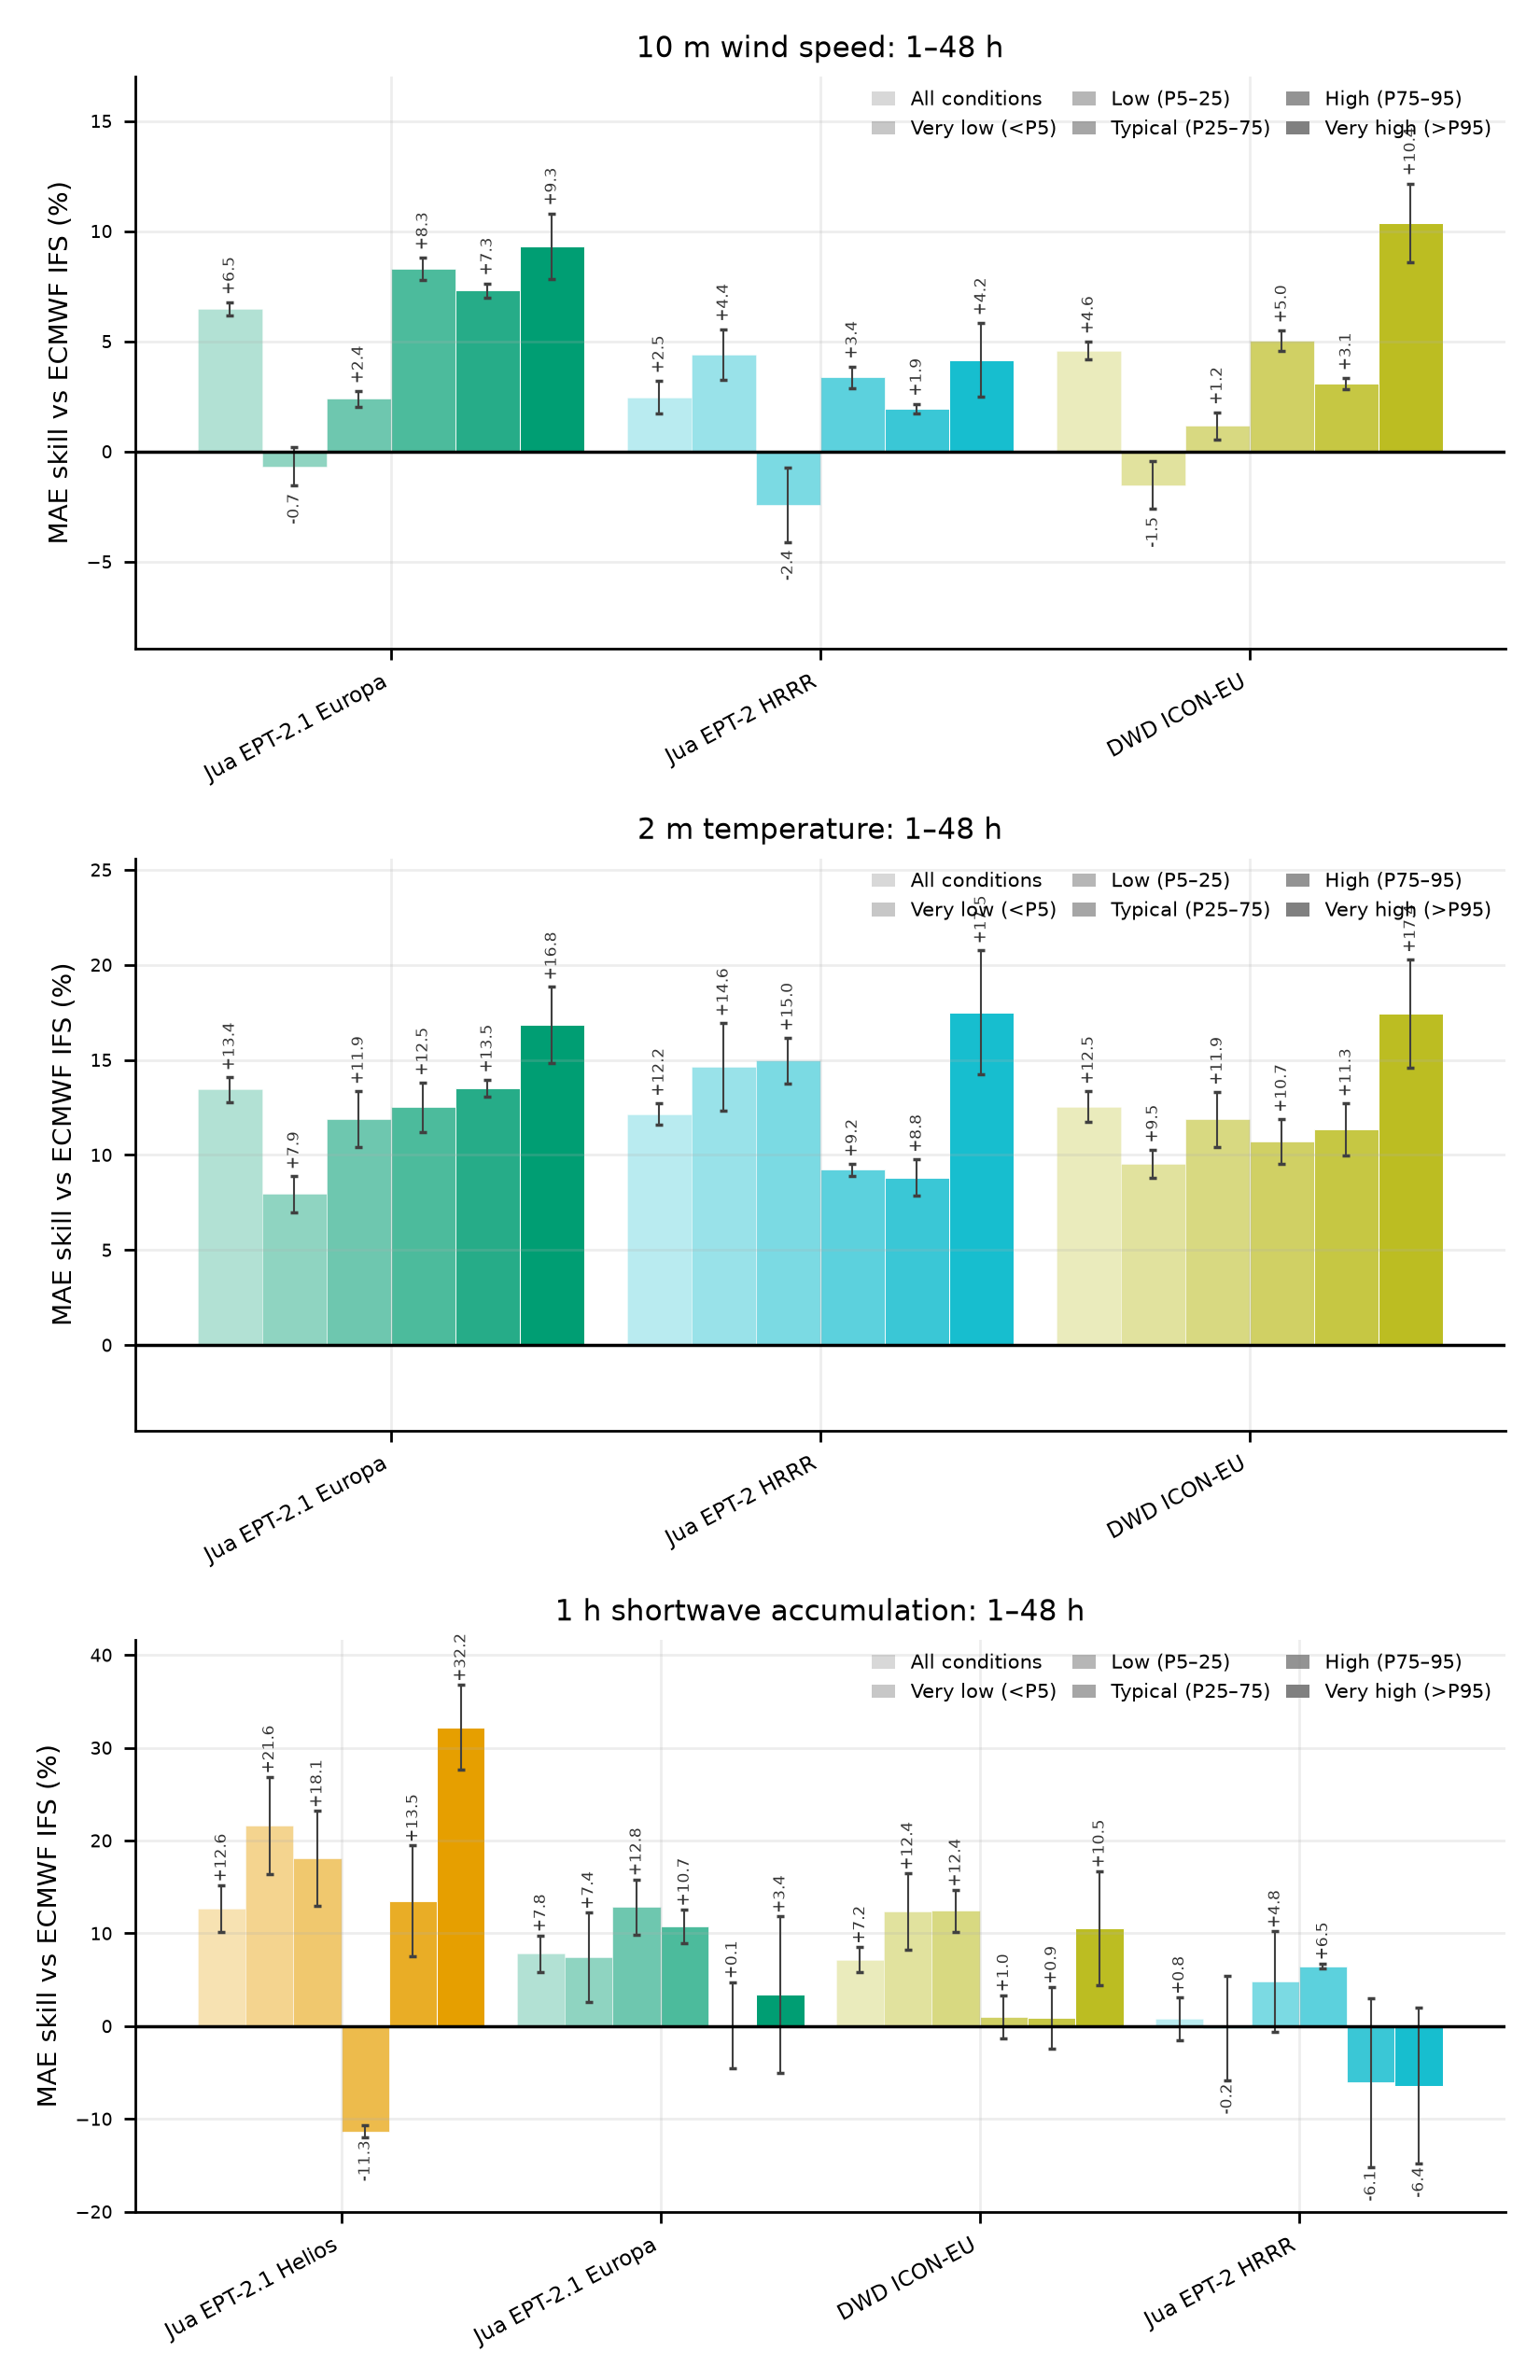
\includegraphics[width=.9\textwidth]{fig8b_track_b_bars.png}
\caption{Track B bias-corrected MAE skill against IFS by
observation-conditioned regime, March--June 2026, 1--48\,h. Uncertainty uses
four monthly blocks.}
\label{fig:trackbbars}
\end{figure}

\begin{table}[h]
\caption{Track B wind MAE skill (\%), 1--48\,h, by regime.}
\label{tab:trackbwind}
\centering\small\resizebox{\textwidth}{!}{\input{tables/t3_track_b_wind_148.tex}}
\end{table}

\begin{table}[h]
\caption{Track B temperature MAE skill (\%), 1--48\,h, by regime.}
\label{tab:trackbtemp}
\centering\small\resizebox{\textwidth}{!}{\begin{tabular}{@{}lrrrrrr@{}}
\toprule
Model & All & $<$P5 & P5--25 & P25--75 & P75--95 & $>$P95 \\
\midrule
Jua EPT-2.1 Europa & +13.4\,(0.6) & +7.9\,(0.9) & +11.9\,(1.5) & +12.5\,(1.3) & +13.5\,(0.4) & +16.8\,(2.0) \\\addlinespace[0.35em]
Jua EPT-2 HRRR & +12.2\,(0.6) & +14.6\,(2.3) & +15.0\,(1.2) & +9.2\,(0.3) & +8.8\,(1.0) & +17.5\,(3.3) \\\addlinespace[0.35em]
DWD ICON-EU & +12.5\,(0.8) & +9.5\,(0.7) & +11.9\,(1.4) & +10.7\,(1.2) & +11.3\,(1.4) & +17.4\,(2.8) \\
\bottomrule
\end{tabular}
}
\end{table}

\begin{table}[h]
\caption{Track B solar MAE skill (\%), 1--48\,h, by regime.}
\label{tab:trackbsolar}
\centering\small\resizebox{\textwidth}{!}{\begin{tabular}{@{}lrrrrrr@{}}
\toprule
Model & All & $<$P5 & P5--25 & P25--75 & P75--95 & $>$P95 \\
\midrule
Jua EPT-2.1 Helios & +12.6\,(2.5) & +21.6\,(5.2) & +18.1\,(5.1) & -11.3\,(0.6) & +13.5\,(5.9) & +32.2\,(4.6) \\\addlinespace[0.35em]
Jua EPT-2.1 Europa & +7.8\,(2.0) & +7.4\,(4.8) & +12.8\,(3.0) & +10.7\,(1.8) & +0.1\,(4.7) & +3.4\,(8.4) \\\addlinespace[0.35em]
Jua EPT-2 HRRR & +0.8\,(2.3) & -0.2\,(5.6) & +4.8\,(5.4) & +6.5\,(0.3) & -6.1\,(9.1) & -6.4\,(8.4) \\\addlinespace[0.35em]
DWD ICON-EU & +7.2\,(1.4) & +12.4\,(4.1) & +12.4\,(2.2) & +1.0\,(2.3) & +0.9\,(3.3) & +10.5\,(6.2) \\
\bottomrule
\end{tabular}
}
\end{table}

\section{Additional methodological details}\label{app:method}

For each model, valid week, initialization hour, and lead, the additive
correction is estimated by pooling station errors from the preceding four
valid weeks. It is one Europe-wide scalar, not a station-specific correction.
Regime labels depend only on the observation and are unchanged by correction.

If $\hat S$ is the full estimate and $\hat S_{(-j)}$ omits month $j$, the
reported standard error is
\[
\operatorname{SE}_{\mathrm{JK}} =
\sqrt{\frac{M-1}{M}\sum_{j=1}^{M}
\left(\hat S_{(-j)}-\overline{\hat S}_{(-\cdot)}\right)^2}.
\]
MAE is pooled linearly by sample count in both the point estimate and each
leave-one-month-out replicate. Track A has $M=10$ and Track B $M=4$.
These values describe sensitivity to months; they are not exact confidence
intervals and do not capture country-level dependence.


\end{document}
